\section{Data}

% Y doan: mo dau phan data bang vai tro cua pipeline trong bai toan.
% Vai tro: dat khung cho ba buoc du lieu chinh va nhan manh bien thuc nghiem nam o connection scope.
This study uses a staged determinant-based pipeline to transform curated NCBI pathogen-surveillance resources\footnote{\url{https://www.ncbi.nlm.nih.gov/pathogens/}} into antibiotic-specific prediction tables. The workflow first restricts both resources to a shared genotype-phenotype cohort, then normalizes determinant-level genotype evidence, and finally reconnects that evidence to phenotype under alternative biological scopes. This structure keeps cohort definition, determinant normalization, and scope-dependent feature construction explicit before the modeling stage begins.

% Y doan: mo ta xu ly phenotype va quy tac loc khang sinh.
% Vai tro: xac dinh label dich va cohort phenotype sach truoc khi noi sang genotype.
\subsection{Phenotype Processing}

% Y doan: chen luu do tom tat cac buoc lam sach phenotype.
% Vai tro: giup nguoi doc nhin nhanh thu tu xu ly truoc khi doc chi tiet bang van ban.
\begin{figure}[h]
\centering
\begin{tikzpicture}[x=1cm,y=1cm,>=stealth, scale=0.92, transform shape]
  \tikzstyle{stepbox}=[draw, rounded corners=3pt, thick, align=center, font=\footnotesize, text width=0.72\textwidth, minimum height=0.8cm, fill=light-gray]
  \tikzstyle{linearrow}=[->, thick]

  \node[stepbox] (raw) at (0,0) {Raw AST records from the NCBI AST Browser};
  \node[stepbox] (cohort) at (0,-1.45) {Step 1: Restrict to isolates shared with the genotype resource through \texttt{BioSample}};
  \node[stepbox] (binary) at (0,-2.9) {Step 2: Keep only \texttt{susceptible}/\texttt{resistant} labels and remove contradictory \texttt{(BioSample, Antibiotic)} pairs};
  \node[stepbox] (duplicate) at (0,-4.35) {Step 3: Resolve remaining duplicate pairs by retaining the lowest MIC observation};
  \node[stepbox] (threshold) at (0,-5.8) {Step 4: Split by antibiotic and apply minimum support thresholds for stable downstream modeling};
  \node[stepbox] (output) at (0,-7.25) {Output: cleaned antibiotic-specific phenotype tables};

  \draw[linearrow] (raw) -- (cohort);
  \draw[linearrow] (cohort) -- (binary);
  \draw[linearrow] (binary) -- (duplicate);
  \draw[linearrow] (duplicate) -- (threshold);
  \draw[linearrow] (threshold) -- (output);
\end{tikzpicture}
\caption[Phenotype-processing workflow.]{Workflow for cleaning AST phenotype records and producing antibiotic-specific phenotype tables.}
\label{fig:phenotype-processing-flow}
\end{figure}

Phenotype processing starts from curated AST records available through the NCBI Pathogen Detection AST Browser\footnote{\url{https://www.ncbi.nlm.nih.gov/pathogens/ast}} and is restricted immediately to isolates that also appear in the genotype resource through a shared \texttt{BioSample} identifier. After cohort alignment, only rows with the required identifying and phenotype fields are retained, and only the labels \texttt{susceptible} and \texttt{resistant} are kept for downstream binary prediction. Any \texttt{(BioSample, Antibiotic)} pair that appears with both labels is removed as contradictory phenotype evidence.

If multiple phenotype rows remain for the same \texttt{(BioSample, Antibiotic)} pair after contradictory labels have been removed, one row is retained by selecting the lowest MIC observation after explicit ordering of measurement signs. This rule makes duplicate resolution deterministic while preserving a consistent and less extreme MIC value within the same final phenotype label, which may be useful if the workflow is later extended beyond binary prediction. The cleaned phenotype data are then split into antibiotic-specific tables because every downstream prediction task is defined at the antibiotic level.

To ensure stable downstream modeling, antibiotic inclusion is filtered using \texttt{MIN\_ANTIBIOTIC\_ROWS = 500} and \texttt{MIN\_CLASS\_COUNT = 100}. The first threshold requires sufficient total support for an antibiotic, and the second requires both resistant and susceptible classes to remain adequately represented. These thresholds are treated as stability requirements for reproducible antibiotic-specific evaluation rather than as exploratory tuning choices.

% Y doan: mo ta xu ly genotype tu dedup den chuan hoa class/subclass.
% Vai tro: bien genotype thô thanh bang determinant da chuan hoa co the noi lai voi phenotype.
\subsection{Genotype Processing}

% Y doan: chen luu do tom tat cac buoc lam sach va chuan hoa genotype.
% Vai tro: giup nguoi doc nam nhanh thu tu xu ly determinant truoc khi doc chi tiet tung quy tac.
\begin{figure}[h]
\centering
\begin{tikzpicture}[x=1cm,y=1cm,>=stealth, scale=0.92, transform shape]
  \tikzstyle{stepbox}=[draw, rounded corners=3pt, thick, align=center, font=\footnotesize, text width=0.72\textwidth, minimum height=0.8cm, fill=light-gray]
  \tikzstyle{linearrow}=[->, thick]

  \node[stepbox] (raw) at (0,0) {Raw MicroBIGG-E determinant records};
  \node[stepbox] (dedup) at (0,-1.45) {Step 1: Remove exact duplicate rows};
  \node[stepbox] (collapse) at (0,-2.9) {Step 2: Collapse to one row per \texttt{(BioSample, Element symbol)}};
  \node[stepbox] (priority) at (0,-4.35) {Step 3: Select the preferred record by method-priority ranking};
  \node[stepbox] (tie) at (0,-5.8) {Step 4: Break remaining ties by subtype preference, then coverage, then identity};
  \node[stepbox] (normalize) at (0,-7.25) {Step 5: Normalize \texttt{Class} and \texttt{Subclass}, including split values and manual mappings};
  \node[stepbox] (output) at (0,-8.7) {Output: one normalized class and one normalized subclass per retained row};

  \draw[linearrow] (raw) -- (dedup);
  \draw[linearrow] (dedup) -- (collapse);
  \draw[linearrow] (collapse) -- (priority);
  \draw[linearrow] (priority) -- (tie);
  \draw[linearrow] (tie) -- (normalize);
  \draw[linearrow] (normalize) -- (output);
\end{tikzpicture}
\caption[Genotype-processing workflow.]{Workflow for deduplicating AMR determinant records and producing normalized class/subclass annotations.}
\label{fig:genotype-processing-flow}
\end{figure}

Genotype processing starts from curated AMR determinant records available through NCBI MicroBIGG-E\footnote{\url{https://www.ncbi.nlm.nih.gov/pathogens/microbigge/}}. In the current experiments, genotype evidence is taken from these curated determinant records rather than generated locally from raw genome data. For new isolates, an equivalent determinant table could be produced by applying AMRFinderPlus to newly sequenced or assembled genomes. Exact duplicate rows are removed first. The remaining table is then collapsed to one row per \texttt{(BioSample, Element symbol)} so that the same determinant is not counted multiple times within one isolate merely because it was detected under multiple reporting methods.

When several rows compete for the same isolate-determinant pair, one preferred record is selected using an explicit method-priority hierarchy: \texttt{EXACT}, \texttt{ALLELE}, \texttt{BLAST}, \texttt{POINT}, \texttt{PARTIAL}, \texttt{PARTIAL\_CONTIG\_END}, and \texttt{HMM}. Remaining ties are broken using subtype-aware preference between \texttt{P} and \texttt{X}, followed by higher coverage and then higher identity. This procedure retains the biologically stronger evidence row while preventing repeated detections from inflating the final feature space.

The raw \texttt{Class} and \texttt{Subclass} annotations are not directly usable because they may contain combined values, mixed capitalization, or ambiguous class-subclass combinations. They are therefore lower-cased, split when multiple class or subclass values are present, and reassigned using observed subclass-to-class mappings derived from simpler cases. To support biologically consistent reassignment in cases where the raw labels remain ambiguous, the normalization procedure also uses a manually curated antibiotic-group reference that summarizes expected relationships between antibiotic subclasses and their broader classes. The fallback value \texttt{unknown} is assigned only when a reliable class-level reassignment cannot be made.

Several rare but biologically meaningful cases require explicit manual normalization support before the \texttt{unknown} fallback. In particular, \texttt{rifampin} is mapped to \texttt{rifamycin}, \texttt{clindamycin} is mapped to \texttt{lincosamide}, and \texttt{trimethoprim-sulfamethoxazole} is decomposed into its component subclasses \texttt{trimethoprim} and \texttt{sulfonamide}. The output of this stage is a normalized genotype table in which each retained row carries exactly one class and one subclass annotation.

% Y doan: mo ta cach noi genotype voi phenotype duoi ba scope.
% Vai tro: dinh nghia bien khoa hoc trung tam cua bai toan va chuan bi du lieu cho rule-based va ML.
\subsection{Genotype-to-Phenotype Connection}

After phenotype cleaning and genotype normalization, each antibiotic-specific phenotype table is linked to the corresponding isolate-level genotype evidence under one of three biological scopes: \textit{strict}, \textit{broad}, or \textit{all}. The resulting feature sets differ only in how broadly determinant evidence is allowed to connect back to the target antibiotic.

Under the \textit{strict} scope, a genotype row is retained only if its normalized subclass matches the narrow lineage of the target antibiotic. Under the \textit{broad} scope, a genotype row is retained if its normalized class belongs to the broader allowed class set of the target antibiotic. This broader match is intended to capture within-family cross-resistance signals that would be lost under exact subclass-level matching. Under the \textit{all} scope, all normalized genotype rows observed for isolates in the target phenotype table are retained regardless of class or subclass. This gives the widest determinant coverage but also allows indirect co-occurrence structure to enter the representation.

\begin{figure}[!htbp]
\centering
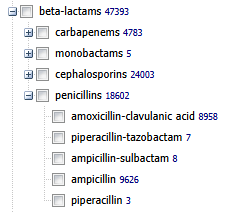
\includegraphics[width=0.45\textwidth]{figures/scope_broad_example}
\caption[Broad-scope example.]{Example of how broad-scope matching connects beta-lactam determinants to related target antibiotics.}
\label{fig:broad-scope-example}
\end{figure}

One important special case is \texttt{trimethoprim-sulfamethoxazole}. For this combination drug, the strict scope is manually expanded so that matching can use biologically meaningful component subclasses rather than a literal compound token only. This makes the strict setting component-aware for that antibiotic and avoids an artificial loss of retained evidence during scope matching.

These three scopes represent progressively wider biological assumptions. A narrow subclass match preserves the most specific interpretation, but it can leave some isolates with sparse retained evidence. A broader family-level match admits within-class signals that may reflect cross-resistance across related drugs. The all-scope representation provides the widest determinant coverage and therefore shows how much predictive signal remains once the biological restriction is removed.
